% !TEX TS-program = xelatex
\documentclass[12pt]{article}

\usepackage[margin=2cm]{geometry}

\usepackage{times}
\usepackage{lineno}
\usepackage[round]{natbib}
\makeatletter
\renewcommand{\@biblabel}[1]{#1.}
\makeatother

\usepackage{graphicx}

\usepackage{url}
\urlstyle{same}

\usepackage[small,compact]{titlesec}

%\titleformat{\section} {\vspace{24pt}\bf\sffamily\MakeUppercase}{\thesection} {0pt} {}
\titleformat{\section} {\vspace{12pt}\bf\large}{\thesection}{0pt}{}
\titleformat{\subsection} {\vspace{6pt}\bf}{\thesubsection} {0pt} {\vspace{-2pt}}
\titleformat{\subsubsection} [runin] {\bf}{\thesubsubsection} {12pt} {}

 
\begin{document}

\title{Blind dating: A phylogenetic approach to dating HIV reservoir sequences}

\author{Joshua Horacsek$^{1,2}$, Jeffrey B. Joy$^2$, \\ Zabrina L. Brumme$^{1,2}$, and Art F.Y. Poon$^{1,2,3}$}
% 1 Simon Fraser University
% 2 BC Centre for Excellence in HIV/AIDS
% 3 University of British Columbia
\baselineskip 22pt
\pagewiselinenumbers

\date{}
\maketitle

\section * {Abstract}

Background: The ability of HIV to persist within latent cellular reservoirs represents a major barrier to cure. 
The timing of establishment of individual viral reservoirs over the infection course could influence their susceptibility to elimination by immune-mediated or therapeutic approaches. 
However, `dating'�� methods to accurately estimate the age of reservoir sequences remain scarce. We propose a simple method to date suspected reservoir sequences using phylogenetic approaches. 

Method: Simulated sequence data for model validation were generated using INDELible version 1.03. 
Published longitudinal clonal sequences from untreated HIV-infected individuals with estimated dates of infection were obtained from the Los Alamos National Laboratory database. 
Maximum-likelihood phylogenies were reconstructed with RaxML. 
Phylogenies were rooted by determining the location of the root that minimized the root-mean-square error between root-to-tip distances and known dates of sampling. 
The root-to-tip distances of latent sequences were mapped to the optimal regression line to estimate their establishment date, which was assumed to precede their sample dates by an unknown amount.
 
Results: We validated the root-to-tip method using simulated data and published longitudinal clonal sequence datasets from untreated HIV-1 infected individuals with known infection dates. 
For each dataset, arbitrary selections of up to 50\% of sequences were handled as latent by censoring their respective sample dates. 
The method accurately recovered these missing sample dates when the phylogeny conformed to a strict molecular clock, as was the case for simulated data %\anote{SOME KIND OF PERFORMANCE METRIC HERE?  MEAN RMSE?}. 
A strict clock model could not be rejected in the majority of empirical within-host data sets. 
When applied to HIV DNA sequences in phylogenies containing dated HIV RNA sequences, we observed that the predicted dates tended to precede dates of sampling, which was consistent with latency %\anote{(MAYBE SOME METRIC HERE LIKE MEAN DISCORDANCE).}

Conclusions:
Given a known phylogeny comprised of longitudinal plasma HIV-1 RNA sequences, the establishment dates of ``��unknown''�� (reservoir) sequences can be reliably estimated when within-host HIV sequence evolution conforms to a molecular clock. 
Future studies will test this method on empirically derived longitudinal within-host HIV deep sequence data and extend the method to work under alternative clock models.

Keywords: 
HIV, Latency, Cellular Reservoirs, Phylogenetics, Linear Regression\\




\section * {Introduction} \label{sec:intro}

A major obstacle along the path of developing HIV cure strategies is the persistence of the virus within latently infected cellular reservoirs \citep{Pace11}. 
Latently infected cells contain integrated HIV DNA and have entered a dormant state in which they not only have a lowered rate of virion production, but may also persist within an individual for several years or more.
Although a patient's viral load can be reduced below detectable levels when that patient is subjected to highly active antiretroviral therapy (HAART), latent reservoirs will eventually reseed an infection if a patient halts treatment \citep{Joos08, Pomerantz03, Richman09}. 
Not much is known about when specific latent reservoirs are established over the course of an infection. 
The chronology of their establishment is of interest as the distribution of ages of the latent virus lineages may provide information concerning the types of adaptations that those lineages may have accumulated. 
Specifically, it may have an influence on how virions produced by those reservoirs will react to immune-mediated and/or therapeutic treatments. 
Previous studies have developed techniques to detect latent lineages by reduced rates of viral evolution \citep{Immonen14} and modelled the population dynamics of different classes of the virus within host \citep{Althaus14}. 
However, there has limited work on estimating when viral lineages suspected of being latent became integrated into the host genome, or qualitatively assessing the distribution of collection-age differences for suspected latent samples.

An HIV-1 population rapidly accumulates genetic diversity over the course of an infection, due to its high mutation rate and short generation time %, and intense selective pressure by the host's immune system 
\citep{Alizon13, Shankarappa99, Rambaut04}. 
Using this extensive sequence diversity, it is possible to reconstruct a phylogenetic tree that represents the descent of virus lineages that have been sampled from a given infection from their common ancestors. 
A phylogeny that is reconstructed by parameterizing a model of molecular evolution \cite[\textit{e.g.}, by maximum likelihood estimation;][]{Felsenstein:1981} solely on the basis of sequence homology has branch lengths in units of expected numbers of substitutions, in which the passage of time is confounded with the rate of evolution.
In other words, a tree that stretches far back in time with a slow rate of evolution will explain a given set of sequences just as effectively as a shallow tree with rapid evolution.  
When lineages are known to be sampled at different times, however, the corresponding tips of the phylogeny can be fixed in time and the rate of evolution between the tips can be estimated directly \citep{Rodrigo99}.
This additional information enables one to rescale a phylogeny in chronological time, which is especially true for HIV-1 populations in which genetic differences can accumulate in weeks or months \citep{Williamson:2003}.
%With an appropriate method of relating evolutionary distance to time (a {\em clock model}), the phylogeny can be re-scaled chronologically, then by fixing the tips to their respective sampling dates, clock ``rates'' can be estimated .
Among the actively replicating HIV lineages within a host, the rate of molecular evolution is fairly consistent over time \citep{Leitner99, Kuhner95, Korber00}.
Consequently, the divergence of these lineages can be adequately approximated by a `strict' molecular clock model in which a single rate of evolution is sustained throughout.
%For sequences originating from the active population of virus, it is not unreasonable to assume that the rate of molecular evolution is relatively constant -- in other words, it adheres to a `molecular clock' model . 
Once a virus lineage becomes integrated into a host genome, however, its rate of evolution becomes negligible relative to the baseline rate in the actively replicating population.
Thus, viral latency effectively halts the molecular evolution of that particular virus lineage until reactivation. 

%Between the active and latent populations, latent cells are then expected to be more genetically different to active lineages than active lineages are among each other.

Viral latency can be manifested by a discordance between a sample's actual collection time and its apparent age based on its sequence divergence from other lineages (Figure \ref{fig:latenttree}). 
Therefore, it may be possible to use phylogenetic analysis to reconstruct the dates that a given virus lineage became latent.
We propose a simple framework to estimate dates of latent reservoirs which assumes that HIV evolution within a host can be adequately modelled by a strict molecular clock, such that the expected number of substitutions per site increases linearly with time \citep{Ho14}. 
%Our method extracts timing information from the phylogenetic relationships between the virus sampled at various time-points along the infection. 
First, we construct a phylogeny relating sequences derived from both cellular HIV DNA and plasma HIV RNA sampled from the same patient.
Next, we parameterize a strict clock by fitting a linear model to the known collection dates of the HIV RNA sequences and the path lengths from the corresponding tips of the phylogeny to the root, which represents the earliest point in time in the phylogeny. 
Since phylogenies reconstructed by the comparative analysis of sequences are typically unrooted, we employ both root-to-tip regression \citep{Korber00} and outgroup rooting methods to estimate the location of the root in the tree. 
We assume that sequences derived from cellular HIV DNA such as that extracted from peripheral blood mononuclear cells (PBMCs) are potentially derived from latent reservoirs. %, and therefore have effectively stopped evolving.
Although sequences derived from plasma HIV RNA may potentially be descended from reactivated latent virus lineages, we assume that this affects only a minority of sequences derived from blood plasma on the time scales represented by the longitudinal data sets in our study (see below).
We used simulated and real longitudinal HIV sequence data sets to evaluate the accuracy of reconstructing tip dates by this approach.
Finally, we applied our method to characterize the integration dates of viral lineages sampled as cellular HIV DNA.

%
%Next, we evaluated the same model on sequence data that was simulated under a model that included viral latency in the form of a variable molecular clock.
%To mimic the types of results we expected from our first test, we used a collection of published longitudinal patient-derived sequence data sets comprising exclusively plasma-derived HIV sequences \citep{McCloskey14} to evaluate the accuracy of date reconstruction for sequences with censored dates. 
%Finally, we tested our methodology on another collection of longitudinal patient-derived data sets comprising both PBMC and plasma sequences. 
%If the molecular clock assumption holds for all sequences, and latency merely implies a ``pause'' in the evolution of a sequence, then the clock should be a reliable source of information for dating latent sequences.




%%%%%%%%%%%%%%%%%%%%%%%% METHODS %%%%%%%%%%%%%%%%%%%%%%%%%%

\section * {Methods} \label{sec:methods}

\subsection * {Simulated Data} \label{subsec:simdata}


% we may need to provide some justification for using BD
To assess the sensitivity of our method, we first simulated HIV sequence data sets without viral latency and evaluated the accuracy of predicting sample collection times from a strict molecular clock model that was fit to a training subset of these data. 
First, we generated phylogenies with 100 tips each under a birth-death model with serial sampling using the sim.bdsky.stt function in the \textit{R} package TreeSim \citep{Boskova14}.
Birth-death models have been applied to studying speciation \citep{Nee:2006} and infectious disease epidemics \citep{Stradler13}, but only recently have been used to model the proliferation of virus lineages in cell populations \citep{Hartfield:2015}.
Lineage birth and death rates were arbitrarily set to $7\times 10^{-3}$ and the sampling probability was set to 0.99.
We used the \textit{R} package NELSI to assign rates of evolution to these trees by drawing values from a Gaussian distribution with a mean rate $\mu = \ 3\times 10^{-4}$ substitutions per generation and standard deviation $\sigma = \ 1\times 10^{-4}$. %; Figure \ref{fig:seedtree} for an example).
To model uncertainty in phylogenetic reconstruction from sequence variation, we simulated sequence evolution along each birth-death tree with INDELible version 1.03 \citep{Indelible09} under an HKY85 \citep{HKY85} model of nucleotide substitution.
Parameters for the substitution model were set to empirical estimates derived from previously published HIV within-host data sets \citep{McCloskey14}. 
Specifically, the stationary distribution was set to 0.42, 0.15, 0.15, 0.28 for the nucleotides A, C, G and T, respectively, and the transition bias parameter was set to 8.5.
A phylogeny was reconstructed from the simulated sequence alignments using the approximate maximum likelihood heuristic implemented in FastTree2 \citep{FastTree10}.
Similar results were obtained with trees reconstructed using RAxML \citep{Raxml14}, which is expected to be more accurate, but can consume orders of magnitude more computational time.
Using this approach, we generated a total of 50 replicate phylogenies without viral latency. 

To simulate phylogenies with latent viral lineages, we used an approach similar to  \citet{Immonen14}. 
However, we used the simplifying assumptions that any sampled virus lineage could undergo no more than one latent period, and that once a lineage entered a latent state, it remained latent until becoming sampled.
For each simulated `latency-free' phylogeny, we chose 50 tips uniformly at random, then shortened their expected number of substitutions and their branch time (the time between the tip, and the tip's parent) by a scalar factor drawn at random from a beta distribution with parameters $\alpha=1$ and $\beta=100$.
We then recorded both the simulated age and simulated collection time and generated sequences along these latent seed trees with INDELible and the same parameters as above. 
For these data, we generated an additional 50 trees with 100 tips each, bringing the total amount of simulated data to 100 trees.


\subsection * {Data Collection} \label{subsec:dcollection}
We collected two distinct sets of data for our experiments. The first we refer to as the {\em plasma} data set, which contains data collected from studies in which only viral RNA in plasma had been collected from individuals. 
The second data set, the {\em mixed} data set, contains sequences from studies in which both viral RNA in plasma and integrated viral DNA from PBMC cells had been collected from the same individual.
Specifically, the {\em plasma} data set \citep{McCloskey14} is a previously assembled and cleaned data set from the Los Alamos HIV Database (\url{http://www.hiv.lanl.gov/}{http://www.hiv.lanl.gov/}). 
This data set contains 335 sets of samples from 232 patients, with over 19,000 sequences \citep{McCloskey14} containing longitudinal samples from the {\em env} region of the HIV-1 genome collected from plasma. 
From this set, we selected treatment naive patients with two or more clonal or single-genome sequences available at each time point, and with a known time-line relative to one of several reference points: HIV infection, seroconversion or presentation of symptomatic seroconversion illness. 
The baseline samples were collected within 186 days of this reference point, and at least one of the subsequent ``follow-up'' time points occurred a minimum of 6 months after baseline.
Patients who had been classified as ``superinfected'' were also excluded \citep{McCloskey14}. 
From this data set, 550 plasma samples from 11 specific patients remained after filtering.


For the {\em mixed} data set, we used the Los Alamos advanced search interface (\url{http://www.hiv.lanl.gov/}{http://www.hiv.lanl.gov/}) to identify subjects who have had both viral RNA from plasma and integrated DNA from PBMC cells collected over various time points. We manually selected individuals from published studies that had well-characterized partial {\em env} sequences. 
There was no condition on the time between sample collection. 
25 individuals were included with plasma samples from at least 2 time points (table \ref{tab:patients}).
A total of 1,249 partial {\em env} sequences from blood plasma, and 1914 partial {\em env} sequences from PBMC cells were used in our analysis. 
We utilized samples from treatment naive individuals from \cite{Shankarappa99, Novitsky09}, samples from individuals that had been treated via HAART from \cite{Llewellyn06}, and samples from individuals that had been on HAART, but ceased treatment \cite{Fischer04}. 
 


\subsection * {Sequence Alignment} \label{subsec:seqalign}
When applicable, we used MUSCLE 3.8.31 \citep{Muscle04} to align the patient-derived sequences, which were then visually inspected and cleaned with AliView \citep{AliView14}. 
Alignments were manually trimmed to the interval in which at least  50\% of sequences within the data set had coverage over each base.
Since the simulated sequence data contained no insertions or deletions, no alignment of these data was necessary. 
Additionally, the plasma data set \citep{McCloskey14} had already been aligned and cleaned, so no further alignment was performed.


\subsection * {Phylogenetic Reconstruction} \label{subsec:phylo}
In all experiments, our reconstructed phylogenies were maximum likelihood phylogenies reconstructed in FastTree2 using the GTR model.
We evaluated two different methods for rooting these trees. The first method is outgroup rooting, in which we chose a taxon that was related to the other taxon, but genetically different enough to resolve the root of the tree, specifically, we chose to root against the HIV-1 B ancestor (\url{http://www.hiv.lanl.gov/}{http://www.hiv.lanl.gov/}) reconstruction
The second method we used to root our trees was a modified version of root-to-tip regression (RTT), in which the tree is systematically re-rooted at every possible internal node, then the root that optimizes an error criterion is selected.
In our experiments, we chose the maximum correlation between the known dates and the evolutionary distance.
Typically, RTT regression uses dates from all tips in its optimization, for this application, we ignored the tips that were undetermined (either censored or otherwise unknown) in the optimization of the root. 
Our synthetic data was only rooted using this modified RTT scheme; for all real data, both outgroup rooting and RTT regression were used to root the phylogeny. 


\subsection * {Date Reconstruction} \label{subsec:daterecon}
We used a general linear model with the normal family to infer the association between the tip dates and sequence divergence from the root. 
The expected amount of evolution was taken to be the response and the sampling dates of the data were taken as the input. 
These models were only calibrated over the uncensored/plasma data for the simulated and real data sets respectively.
We then used the linear model to predict the dates of the latent/unknown sequences.
To screen for data that were amenable to our analysis, we used the nested log ratio test \citep{Ho14}. 
Our null model was a linear model with zero slope over the expected amount of evolution over time. 
We rejected any sequence data sets whose phylogeny couldn't reject the null model with threshold $\alpha=0.01$, since this implied a lack of phylogenetic signal.


\subsection * {Experiments} \label{subsec:experiments}
We used three error metrics to assess our methodology: the mean square error for predicted date, as well as the mean and median difference between the predicted date and sampling date, where difference defined as simply the predicted date minus the observed date.
Before any analysis was done, all tip dates were re-scaled to lie between $0$ and $1$ to facilitate comparisons among longitudinal data sets. 
Using the formula  $$ t_{normalized} = \frac{t - \min(\bf{t}) }{ \max{(\bf{t})} - \min{(\bf{t}})}$$ where $t$ is the the unscaled time of any tip, and $\bf{t}$ is the vector of all tip dates for a given tree, we call this {\em normalized time}. Our error metrics were then calculated from these normalized times, giving normalized mean square error, normalized mean difference, and normalized median difference. 

Our first validation experiment on simulated data was preformed as such: first we choose 50\% of the tips of a simulated phylogeny and censored those dates, we next used our  modified RTT regression \citep{APE} on the remaining data to calibrate the phylogeny's molecular clock. 
For each censored date we reconstructed the expected date using the regression model defined above, then collected the three error metrics above.
For the simulated latent data, we collected the normalized mean square error, normalized mean difference, and normalized median difference. 
We also collect these for the known ``archival'' date.

To evaluate the effectiveness of this methodology on real data, we utilized our {\em plasma} data set \citep{McCloskey14} and performed similar experiments. 
As before, we censored 50\% of their known sampling dates then reconstructed the censored dates using a linear model calibrated over the uncensored dates. 
We also performed this experiment with RTT regression rooting and out-group rooting. The goal of this experiment was to parallel the type of results of the first experiment on simulated data. 

Finally, we looked at our {\em mixed} data set comprised of both PBMC and plasma data. 
We used both RTT regression and out-group rooting to root the phylogeny, then calibrated a clock to the known plasma sampling dates and reconstructed the expected age of the sequences for all patients who could reject the null model (Section \ref{subsec:hypot}). 
Here we only collected the normalized errors between the prediction and the collection.



\section * {Results} \label{sec:results}



\subsection * {Model Validation} \label{sec:sim_results}
Figure \ref{fig:results1} shows our model validation results over our synthetic data -- here we censor 50\% of the dates, and attempt to reconstruct them. 
Under the assumption of a strict molecular clock (that evolution is linearly related to time) the clock is a reliable source of information for these simulations.
Figure \ref{fig:results1} A shows this result for the synthetic data with no latent behaviour.
Averaged over all simulated data sets, the mean square error was $3.0\times 10^{-3}$, and the average median and mean difference were 0 and $5.0\times 10^{-5}$ respectively. 
Quantitatively, the censored data points are close to the regression line, and the difference density is heavily peaked around 0. 

Figure \ref{fig:results1} B shows different results for the latent simulations -- here we censor 50\% of the dates, attempt to reconstruct them, then compare them to the simulated collection dates. 
In this case, averaged over all simulated data sets, the mean square error was $7.1\times 10^{-3}$, and the average median and mean difference were $4.0\times 10^{-2}$ and $5.1\times 10^{-2}$ respectively. 
This bias is expected, as the errors were calculated between the simulated collection times -- not the simulated archival times.
More quantitatively, we expect the density plot to be shifted to the right (as it is in figure \ref{fig:results1} B) as this suggests that sequences are older than their sampling dates.
When we performed the same analysis against the simulated archival times, the results were nearly identical to the results without any latent data, suggesting that we can recover the dates of latent sequences provided an accurate clock.

For our final validation, we took the same strategy as the first validation on synthetic data, and applied it to our {\em plasma} data set -- we censored known sampling dates, then attempted to reconstruct them (Figure \ref{fig:results2} C shows this when the phylogenies have been rooted with outgroup rooting). 
Averaged over all simulated data sets, the mean square error was $1.7\times 10^{-1}$, and the absolute value of average median and mean difference were $2.1\times 10^{-4}$ and $1.9\times 10^{-2}$ respectively. 
The density plot shows similar behavior to that of the synthetic data, except with a wider distribution, and more variation. 


\subsection * {Application} \label{sec:mixed_data}

Finally, we tested our methodology on the {\em mixed} data set.
Figure \ref{fig:results2} D shows the regression over the plasma calibration dates the plasma collection dates. 
In this case, we do not know the actual date of archival, however, the superposition of the difference density plots shows similar behavior to that of the latent simulated data.

With respect to the sampling time, over all individuals, the mean square error was $4.9\times 10^{-2}$, and the absolute value of average median and mean difference were $2.4\times 10^{-2}$ and $4.7\times 10^{-3}$.

Individuals that had received treatment at some point generally failed the hypothesis test -- there was only one patient that did not -- these individuals were not included in the above analysis. 


%%%%%%%%%%%%%%%%%%%%%%%%%%%%%%%%%%%%%%
\section * {Discussion} \label{sec:discuss}
The results concerning the simulated data were highly consistent with expectations. 
The more a phylogeny adheres to a molecular clock, the more accurate predictions made from it will be -- the simulated data is very well informed, and the phylogenies and their clocks are well resolved by the maximum likelihood tree estimate. 
Since latency is akin to ``pausing'' the evolution of a sequence, and evolution is assumed to be clock-like when sequences are not ``paused'', it's also not surprising that the latent simulated data could be reconstructed with low error. 

The results from the {\em plasma} data-set are also expected. 
Each patient from our plasma data-set showed evidence of a molecular clock, so the ability to reconstruct known dates came as no surprise. 
However, the reconstruction error was higher than that of the simulated data, which is expected for data that come from a real biological process.

Quantitatively, it's difficult to assess the accuracy of the reconstructions within the {\em mixed} data set. 
Many patients show evidence of latency in their regression plots (see the regression plot in Figure \ref{fig:results2} D) but it's unclear what the general pattern is (if any) for the distribution of the error metrics. 
Moreover, it's not possible to know the actual error for this data set, as that would require us to know the date at which a sequence became latent. 
We also observed an interesting sigmoidal pattern in many of the patients in this case.
However, we do note that most treated patients failed the hypothesis testing, implying that samples after treatment should be ignored in any analysis with this methodology.

Typically, we also observed that the rooting method had very little effect on the errors (the supplemental material has Figure \ref{fig:results2} replicated for RTT rooting). 
We did, however, identify a case in which RTT rooting fails over outgroup rooting (Figure \ref{fig:degenerate_example} shows an example of this). 
Specifically, it's possible for the calibration dates to provide insufficient data to resolve the root of the tree. 
We theorize that this is, for patient 820, because their calibration samples are strongly localized in time, which allows too much freedom (temporally) over the possible roots of the tree. 

%We did not attempt to use BEAST \citep{BEAST} to reconstruct any phylogenies from our data.
%Leaving dates unspecified on the number of tips would have drastically increased the dimensionality of the problem, and we would therefore need a prohibitively large amount of samples from the MCMC chain to assure convergence to the posterior distribution.



We also noticed that the patients who had begun treatment (regardless of whether or not they regressed) typically failed the hypothesis testing. Upon analysing the clocks of these individuals, they showed two trends. 
The first trend, in patients who had regressed after treatment, was the ``resetting'' of the molecular clock -- that is, after treatment started, the clock was set to a previous point in time, then continued as it had before after treatment failed. 
For patients who had successfully been treated, there appeared to be an emergence of a clock with near zero slope after treatment.
This suggests that after a patient begins treatment, the assumption of a molecular clock  is not valid over the whole temporal range of the phylogeny. 



%\section * {Conclusion} \label{sec:conclusion}
In this work we showed that a phylogeny's clock, when reliable, is a valuable source of information with respect to dating sequences that are suspected to show latent behaviour in patients infected with HIV-1. 
Through simulation, we built phylogenies that adhered to clock-like behaviour, with and without latent sequences.
From those, were able to reliably reconstruct dates for both active and latent sequences, rooting the trees via root-to-tip regression.
Then, using real data, we performed analogous reconstructions, using both root-to-tip regression and outgroup rooting, and showed similar results.

However, there are ways in which this method could be improved. 
These results hinge on the strong assumption of a molecular clock over the data, which is not always true. 
It may be possible to adapt a maximum likelihood relaxed clock methodology with this approach, giving more flexibility over noisy or unreliable data. 
Additionally, we would like to apply the methodology to next gen sequence data -- we would like to see if mass amounts of short read data contain sufficient information to calibrate the clock.


%\section{Acknowledgments} \label{sec:ackn}
%The authors would like to thank --.

\clearpage

\bibliographystyle{plainnat}
\bibliography{blind-dating}


\clearpage

%%%%%%%%%%%%%%%  FIGURES  %%%%%%%%%%%%%%%

\section * {Figures}

\begin{figure}[ht] \label{fig:latenttree}
	\centering
	%\scalebox{5}{%LaTeX with PSTricks extensions
%%Creator: inkscape 0.91
%%Please note this file requires PSTricks extensions
\psset{xunit=.5pt,yunit=.5pt,runit=.5pt}
\begin{pspicture}(85,53)
{
\newrgbcolor{curcolor}{0 0 0}
\pscustom[linewidth=0.38699999,linecolor=curcolor]
{
\newpath
\moveto(77.921134,4.13898)
\lineto(5.1912118,4.13898)
\lineto(5.1912118,20.207747)
}
}
{
\newrgbcolor{curcolor}{0 0 0}
\pscustom[linewidth=0.38699999,linecolor=curcolor]
{
\newpath
\moveto(65.799478,25.564002)
\lineto(29.434525,25.564002)
\lineto(29.434525,36.276514)
}
}
{
\newrgbcolor{curcolor}{0 0 0}
\pscustom[linewidth=0.38699999,linecolor=curcolor]
{
\newpath
\moveto(41.556173,46.989025)
\lineto(29.434525,46.989025)
\lineto(29.434525,36.276514)
}
}
{
\newrgbcolor{curcolor}{0 0 0}
\pscustom[linewidth=0.38699999,linecolor=curcolor]
{
\newpath
\moveto(29.434525,36.276514)
\lineto(5.1912118,36.276514)
\lineto(5.1912118,20.207747)
}
}
{
\newrgbcolor{curcolor}{0 0 0}
\pscustom[linewidth=0.38699999,linecolor=curcolor]
{
\newpath
\moveto(4.4639148,20.207747)
\lineto(5.1912118,20.207747)
}
}
{
\newrgbcolor{curcolor}{0 0 0}
\pscustom[linestyle=none,fillstyle=solid,fillcolor=curcolor]
{
\newpath
\moveto(81.87934379,5.47198716)
\lineto(81.87934379,5.02049697)
\curveto(81.73520608,5.15474288)(81.58117656,5.25507403)(81.41725524,5.32149043)
\curveto(81.25474704,5.38790683)(81.08164047,5.42111503)(80.89793554,5.42111503)
\curveto(80.53617814,5.42111503)(80.25920764,5.31018551)(80.06702402,5.08832648)
\curveto(79.8748404,4.86788057)(79.77874859,4.54851662)(79.77874859,4.13023462)
\curveto(79.77874859,3.71336575)(79.8748404,3.3940018)(80.06702402,3.17214277)
\curveto(80.25920764,2.95169685)(80.53617814,2.84147389)(80.89793554,2.84147389)
\curveto(81.08164047,2.84147389)(81.25474704,2.87468209)(81.41725524,2.94109849)
\curveto(81.58117656,3.00751489)(81.73520608,3.10784604)(81.87934379,3.24209195)
\lineto(81.87934379,2.79484111)
\curveto(81.72955362,2.69309684)(81.5705782,2.61678864)(81.40241754,2.5659165)
\curveto(81.23566999,2.51504437)(81.05903063,2.4896083)(80.87249947,2.4896083)
\curveto(80.39345355,2.4896083)(80.01615188,2.63586569)(79.74059449,2.92838046)
\curveto(79.4650371,3.22230834)(79.3272584,3.6229264)(79.3272584,4.13023462)
\curveto(79.3272584,4.63895596)(79.4650371,5.03957402)(79.74059449,5.33208879)
\curveto(80.01615188,5.62601668)(80.39345355,5.77298062)(80.87249947,5.77298062)
\curveto(81.06185686,5.77298062)(81.23990933,5.74754455)(81.40665688,5.69667242)
\curveto(81.57481755,5.6472134)(81.73237985,5.57231831)(81.87934379,5.47198716)
\closepath
}
}
{
\newrgbcolor{curcolor}{0 0 0}
\pscustom[linestyle=none,fillstyle=solid,fillcolor=curcolor]
{
\newpath
\moveto(67.94040944,25.49054575)
\lineto(67.94040944,24.41103725)
\lineto(68.57982581,24.41103725)
\curveto(68.79428027,24.41103725)(68.95281869,24.45511225)(69.05544107,24.54326224)
\curveto(69.15937912,24.63272791)(69.21134815,24.76889991)(69.21134815,24.95177825)
\curveto(69.21134815,25.13597227)(69.15937912,25.27148644)(69.05544107,25.35832076)
\curveto(68.95281869,25.44647075)(68.79428027,25.49054575)(68.57982581,25.49054575)
\lineto(67.94040944,25.49054575)
\closepath
\moveto(67.94040944,26.70227923)
\lineto(67.94040944,25.81420095)
\lineto(68.53048813,25.81420095)
\curveto(68.72520752,25.81420095)(68.86993138,25.85038191)(68.96465973,25.92274385)
\curveto(69.06070376,25.99642145)(69.10872577,26.10825353)(69.10872577,26.25824009)
\curveto(69.10872577,26.40691097)(69.06070376,26.51808522)(68.96465973,26.59176282)
\curveto(68.86993138,26.66544043)(68.72520752,26.70227923)(68.53048813,26.70227923)
\lineto(67.94040944,26.70227923)
\closepath
\moveto(67.54176097,27.02988145)
\lineto(68.56009074,27.02988145)
\curveto(68.86401086,27.02988145)(69.0982004,26.96672921)(69.26265934,26.84042474)
\curveto(69.42711828,26.71412028)(69.50934775,26.53453111)(69.50934775,26.30165725)
\curveto(69.50934775,26.12141025)(69.46724626,25.97800205)(69.38304328,25.87143266)
\curveto(69.29884031,25.76486326)(69.17516718,25.69842185)(69.01202391,25.67210842)
\curveto(69.20805897,25.63000693)(69.36001903,25.54185694)(69.4679041,25.40765844)
\curveto(69.57710484,25.27477562)(69.6317052,25.10834317)(69.6317052,24.90836109)
\curveto(69.6317052,24.64522679)(69.54223954,24.44195553)(69.36330821,24.29854734)
\curveto(69.18437688,24.15513914)(68.92979444,24.08343504)(68.59956088,24.08343504)
\lineto(67.54176097,24.08343504)
\lineto(67.54176097,27.02988145)
\closepath
}
}
{
\newrgbcolor{curcolor}{0 0 0}
\pscustom[linestyle=none,fillstyle=solid,fillcolor=curcolor]
{
\newpath
\moveto(68.8325765,47.98448198)
\lineto(68.33071752,46.62360158)
\lineto(69.33626709,46.62360158)
\lineto(68.8325765,47.98448198)
\closepath
\moveto(68.62377386,48.34897081)
\lineto(69.04321075,48.34897081)
\lineto(70.08539237,45.6143888)
\lineto(69.70075592,45.6143888)
\lineto(69.45165803,46.31589242)
\lineto(68.21898978,46.31589242)
\lineto(67.96989189,45.6143888)
\lineto(67.57976063,45.6143888)
\lineto(68.62377386,48.34897081)
\closepath
}
}
{
\newrgbcolor{curcolor}{0 0 0}
\pscustom[linewidth=0.39463133,linecolor=curcolor,linestyle=dashed,dash=0.7892628 0.7892628]
{
\newpath
\moveto(41.217255,46.97727)
\lineto(65.885506,46.9308)
}
}
\rput(42,52){\psscalebox{0.3}{$t$}}
\rput(66,52){\psscalebox{0.3}{$t^\prime$}}
\end{pspicture}
}
	\includegraphics{figures/latency-scheme}
	\caption[]{ 
	Reconstructing the time that a viral lineage entered a latent state from sequence variation.  
	A dashed line illustrates the linear relationship between the divergence of lineages from the ancestral sequence at the root ($y$-axis) and passage of time since the root ($x$-axis).
	Grey lines represent the reconstructed phylogenetic relationships among these lineages.
	The lineages were sampled (open circles) at three points in time.
	%Above is a time calibrated phylogeny with three taxa, the dotted line in is an example of latency. 
	One of these lineages had become latent at an earlier point in time (red hexagon).
	This lineage subsequently underwent negligible molecular evolution until it was sampled as integrated viral DNA (dashed circle).
	If the relationship between sequence divergence and time is sufficiently linear, then the time that the lineage became latent can be inferred from its sequence.
	%Sequence A was archived at time $t$, and was collected at the same time as sequence B, at time $t^\prime$ (a drift of $t^\prime - t$ is expected).
	%If the molecular clock assumption holds true, the MRCA is known, and B and C are reliable time-points, then the date at $t$ can be inferred from from the expected amount of evolution for B from the root.
	}
\end{figure}

\begin{figure}[p] \label{fig:results1}
	\centering
	\includegraphics[width=\textwidth]{figures/simulated.pdf} 
	\includegraphics[width=\textwidth]{figures/simulated_latent.pdf}\\
	\caption[Simulated Data]{On the left of each case is a plot of evolutionary distance vs time, the right is a the super position of density estimates (of normalized error) for each phylogeny (with kernel bandwidth = $0.15$). The red line on the density plot is the mean error, and the black line is the median error. }
\end{figure}

\begin{figure}[ht] \label{fig:results2}
	\centering
	\includegraphics[width=\textwidth]{figures/ancre.pdf}
	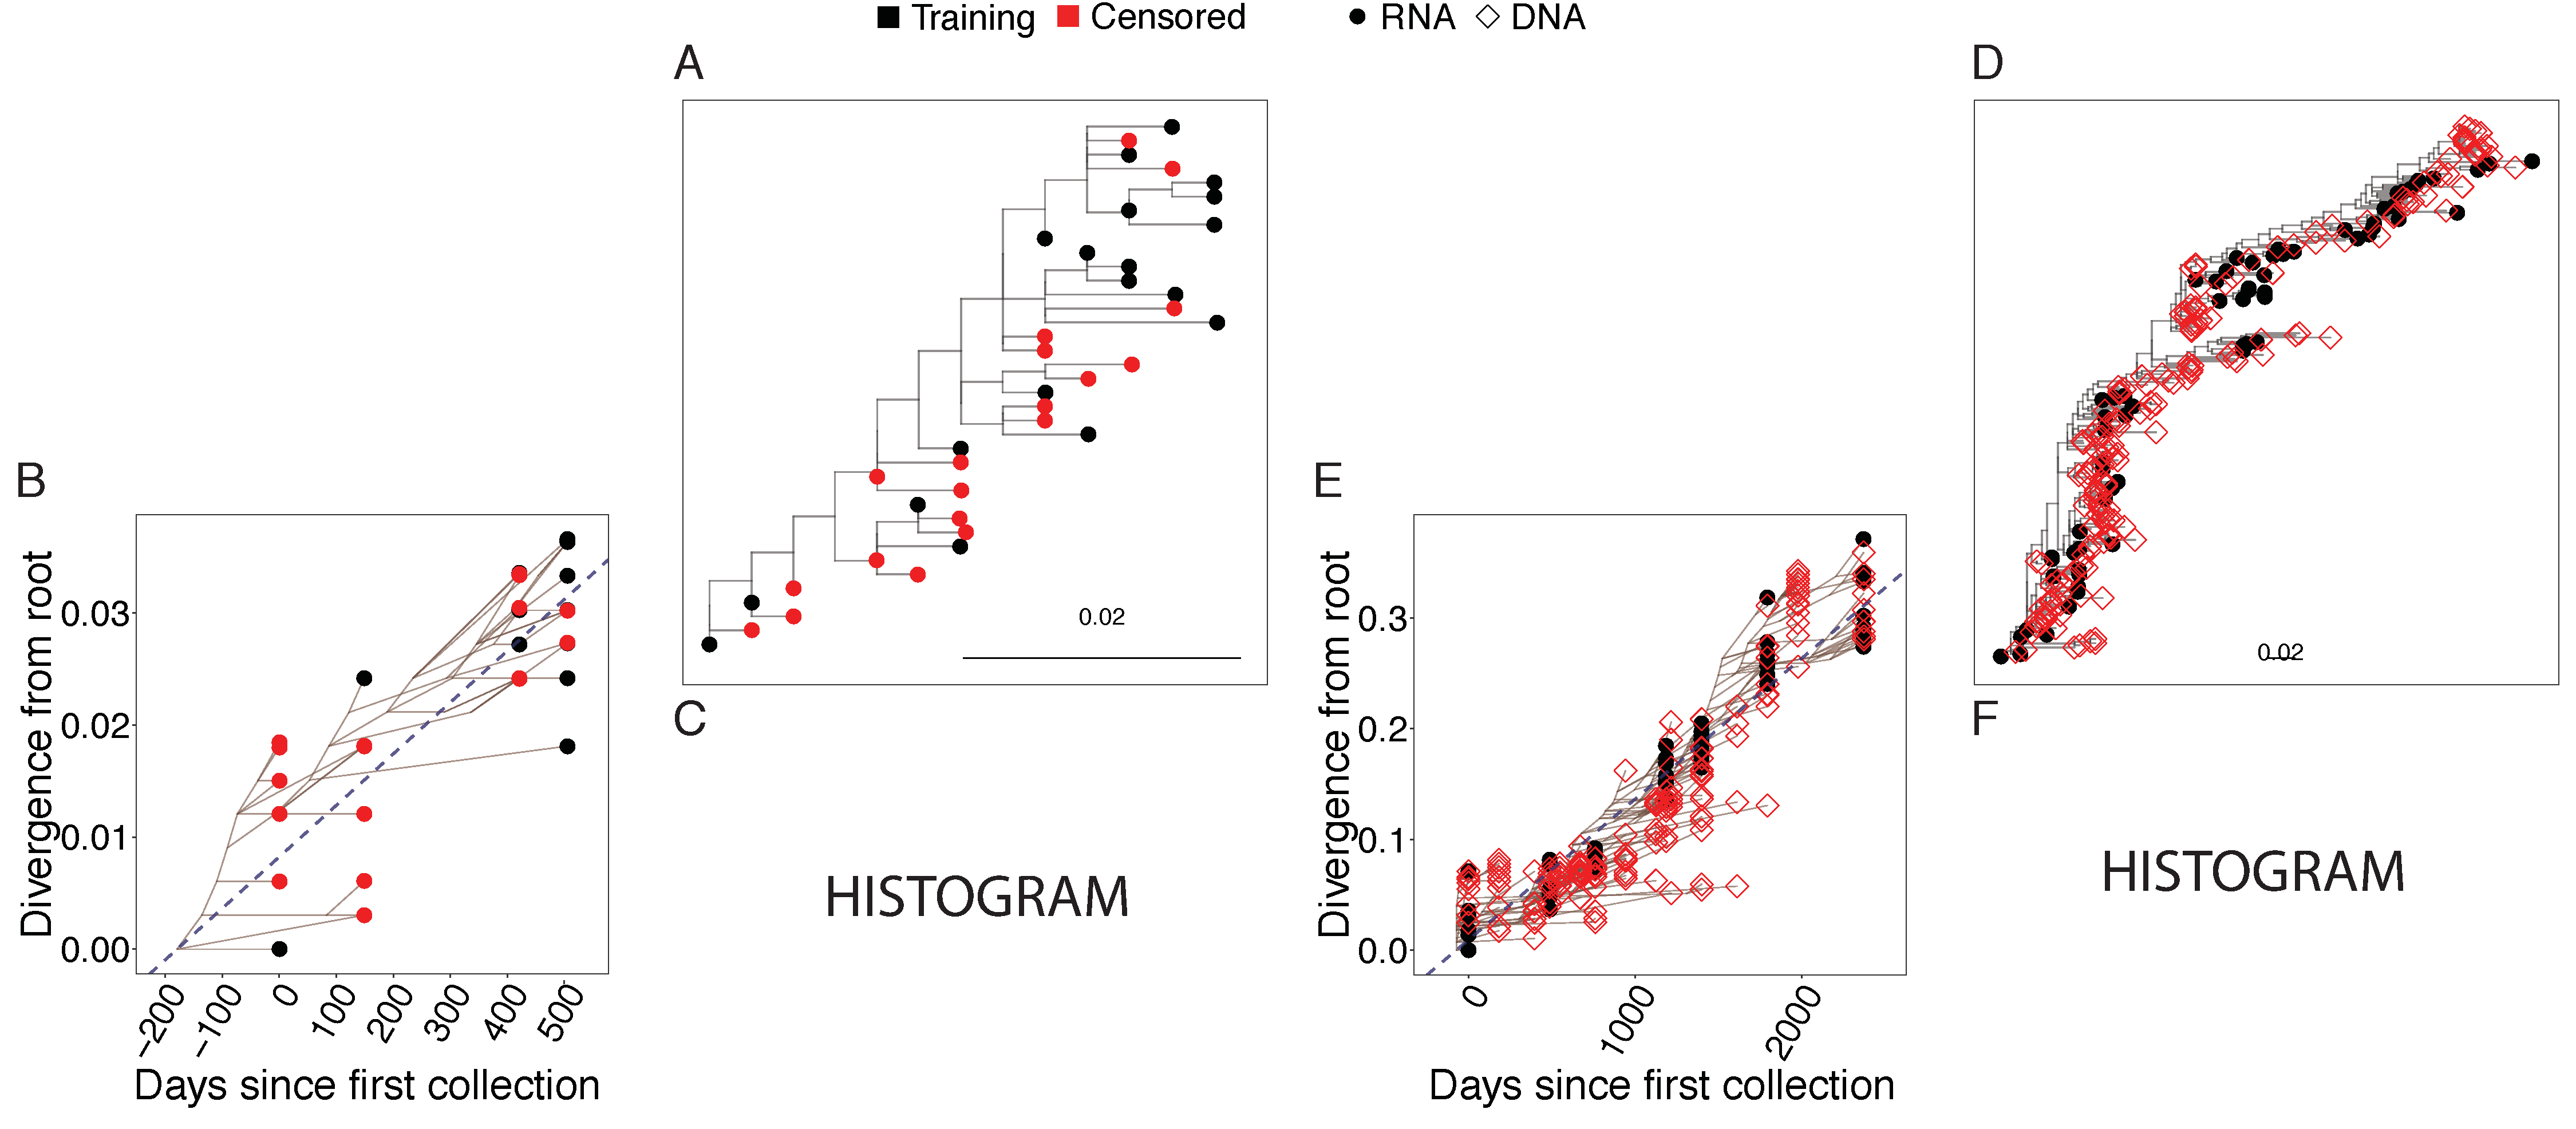
\includegraphics[width=\textwidth]{figures/lanl.pdf}
	\caption[Examples]{This figure is as the previous, except for the real data.
The phylogenies in these cases have been rooted with outgroup rooting}
\end{figure}

\begin{figure*}[ht] \label{fig:degenerate_example}
	\centering
	\includegraphics[scale=0.425]{figures/rtt.pdf} \\
	\caption[Example of bad root]{Root to tip rooting fails due to insufficient temporal resolution at the root}
\end{figure*}


\clearpage

%%%%%%%%%%%%%%%  TABLES  %%%%%%%%%%%%%%%

\section * {Tables}

\begin{table*}[!ht]
\def\arraystretch{1.3}%
\begin{center}
\begin{tabular}{llrrrrrr} 

Reference & Patient ID & \multicolumn{3}{c}{Sequences} & \multicolumn{3}{c}{Time points}\\ 
 &  & Plasma & PBMC & Total & Plasma & PBMC & Total\\
\hline
\cite{Shankarappa99} & 820 &       50 &       87 &      137 &        5 &       10 &       15  \\
& 821 &      76 &      192 &      268 &        7 &       17 &       17   \\ 
& 822 &      32 &       98 &      130 &        3 &       10 &       10   \\ 
& 824 &     100 &      107 &      207 &        7 &        9 &       13   \\ 
& 10137 &     24 &      106 &      130 &        2 &       10 &       12  \\ 
& 10138 &     82 &      119 &      201 &        6 &       13 &       16  \\
& 10586 &     16 &      121 &      137 &        2 &       12 &       14  \\ 
& 13889 &    151 &      132 &      283 &       13 &       14 &       18  \\ 
 \cite{Fischer04} & 10769 &    229 &       96 &      325 &       10 &        4 &       11  \\ 
& 10770 &    190 &       31 &      221 &       11 &        2 &       11  \\ 
\cite{Llewellyn06} & 16616 &     16 &       95 &      111 &        2 &        5 &        5  \\ 
& 16617 &     16 &       89 &      105 &        2 &        5 &        5  \\ 
& 16618 &     25 &       75 &      100 &        2 &        5 &        6  \\ 
& 16619 &     13 &       60 &       73 &        2 &        6 &        6  \\ 
\cite{Novitsky09} & 34382 &     37 &        5 &       42 &        3 &        1 &        4  \\ 
& 34391 &     13 &       38 &       51 &        3 &        5 &        6  \\ 
& 34393 &     25 &       74 &       99 &        2 &        6 &        7  \\ 
& 34396 &      23 &       46 &       69 &        2 &        5 &        5 \\ 
& 34397 &      26 &       25 &       51 &        2 &        2 &        4  \\ 
& 34399 &      61 &       88 &      149 &        5 &        9 &       12  \\ 
& 34400 &      54 &       23 &       77 &        4 &        1 &        5  \\ 
& 34405 &      27 &       29 &       56 &        3 &        2 &        4  \\ 
& 34408 &       5 &       73 &       78 &        2 &        8 &        8 \\ 
& 34410 &      35 &       60 &       95 &        2 &        6 &        6 \\ 
& 34411 &      25 &       43 &       68 &        3 &        3 &        6   \\ \hline
\end{tabular}
\end{center}
  \caption{Summary of all the patient data collected from the HIV LANL database -- Patient ID corresponds to the Los Alamos database's Patient ID \citep{LosAlamos}.
   }\label{tab:patients} 
\end{table*}



\end{document}


